\section{Introducción a la Demostración}
Una \textbf{demostración} es un argumento lógico que establece la verdad de un enunciado matemático.
Se construye a partir de axiomas, definiciones y teoremas previamente probados.

En clases anteriores, hemos explorado las \textbf{reglas de inferencia} en lógica, que nos permiten derivar conclusiones a partir de premisas utilizando razonamiento formal. Estas reglas, como el \textit{Modus Ponens}, \textit{Modus Tollens}, la transitividad de la implicación, entre otras, constituyen la base fundamental de las demostraciones matemáticas. Ahora, aplicaremos estas reglas de manera menos estructurada en distintas estrategias de demostración para establecer formalmente la validez de proposiciones matemáticas.

Las demostraciones pueden ser formales o informales. Las \textbf{demostraciones formales} detallan cada paso con precisión matemática, pero suelen ser largas y difíciles de seguir. En la práctica, las demostraciones suelen ser más informales y omiten detalles obvios para los lectores familiarizados con la teoría.

\subsection{Clasificación de Teoremas y Resultados Matemáticos}

En matemáticas, los resultados se clasifican en:

\begin{itemize}
    \item \textbf{Teorema}: Un resultado matemático importante con una demostración no trivial.
    \item \textbf{Lema}: Un resultado auxiliar que facilita la demostración de un teorema.
    \item \textbf{Proposición}: Un resultado matemático relevante pero de menor importancia que un teorema.
    \item \textbf{Corolario}: Un resultado que sigue inmediatamente de un teorema.
    \item \textbf{Conjetura}: Una afirmación que se cree verdadera pero que aún no ha sido probada.
\end{itemize}

\subsection{Métodos de Demostración}

Muchos teoremas tienen la forma $\forall x ~ (P(x) \to Q(x))$, donde $P$ representa la hipótesis y $Q$ la conclusión. Para probar esta afirmación, existen diversas estrategias:

\subsubsection{Demostración Directa}

Se parte de la hipótesis $P$ y se deduce la conclusión $Q$ mediante una secuencia lógica de pasos.

\begin{exampleblock}{Ejemplo: Demostrar que si $n$ es impar\text{,} entonces $n^2$ también es impar.}

\begin{proof}
    Si $n$ es impar, entonces se puede escribir como $n = 2k + 1$ para algún entero $k$. Elevando al cuadrado:
    \[
    n^2 = (2k+1)^2 = 4k^2 + 4k + 1 = 2(2k^2 + 2k) + 1.
    \]
    Como el resultado es de la forma $2m + 1$, donde $m$ es un entero, $n^2$ es impar.
\end{proof}
\end{exampleblock}

\subsubsection{Demostración por Contraposición}

En lugar de demostrar $P \to Q$, se demuestra su contrapartida lógica: $\neg Q \to \neg P$.

\begin{exampleblock}{Ejemplo: Si $3n+2$ es impar\text{,} demostrar que $n$ es impar. }

\begin{proof}
    Demostramos la contraposición: si $n$ es par, entonces $3n+2$ es par.
    Si $n = 2k$, entonces $3n+2 = 3(2k) + 2 = 6k+2 = 2(3k+1)$, que es par.
    Por lo tanto, si $3n+2$ es impar, entonces $n$ es impar.
\end{proof}
\end{exampleblock}

\subsubsection{Demostración por Análisis de Casos}

Se divide el problema en varios casos y se demuestra el resultado en cada uno de ellos.

\begin{exampleblock}{Ejemplo: Probar que si $n$ no es múltiplo de 3\text{,} entonces $3 \mid (n^2 - 1)$.}

\begin{proof}
    Si $n$ no es múltiplo de 3, puede ser de la forma $3k+1$ o $3k+2$.
    \begin{itemize}
        \item Si $n = 3k+1$, entonces $n^2 = 9k^2 + 6k + 1$, y $n^2 - 1 = 3(3k^2 + 2k)$, múltiplo de 3.
        \item Si $n = 3k+2$, entonces $n^2 = 9k^2 + 12k + 4$, y $n^2 - 1 = 3(3k^2 + 4k + 1)$, múltiplo de 3.
    \end{itemize}
    En ambos casos, $3 \mid (n^2 - 1)$.
\end{proof}
\end{exampleblock}

\subsubsection{Demostración por Contradicción}

Se asume que la afirmación es falsa y se llega a una contradicción. Es decir, en lugar de demostrar $P$, se demuestra $\neg P \to \bot$

\begin{exampleblock}{Ejemplo: Demostrar que no existe un número racional menor que todos los racionales positivos.}

\begin{proof}
    Supongamos que existe un número racional $r$ tal que $r$ es el menor de todos los racionales positivos.
    Entonces, $r/2$ también es un número racional positivo y es menor que $r$, lo que contradice la suposición.
    Por lo tanto, tal número no puede existir.
\end{proof}
\end{exampleblock}

Una proposición de la forma $p \rightarrow q$ también puede ser probada por
contradicción. Basta derivar una contradicción a partir de $p \wedge \neg q$.

\subsection{Conclusión}

Las demostraciones matemáticas son fundamentales en la matemática discreta y en toda la disciplina matemática.
Cada técnica tiene su lugar y su utilidad dependiendo de la estructura del teorema a demostrar. La práctica en la construcción de demostraciones ayuda a mejorar la capacidad de razonamiento lógico y la creatividad matemática.

\subsection{Problemas Propuestos}

\begin{enumerate}
    \item Probar que la suma de dos números impares siempre es par.
    \item Demuestre por contraposición que si $n = ab$, donde ambos $a$ y $b$ son reales positivos, entonces $a \leq \sqrt{n}$ o $b \leq \sqrt{n}$.
    \item Usar el método de contradicción para demostrar que $\sqrt{3}$ es irracional.
    \item Probar por contradicción que si $a$ y $b$ son reales positivos, entonces $a+b \geq 2\sqrt{ab}$
    \item Probar que para todo entero $n$, si $n^2$ es par, entonces $n$ es par.
    \item Probar por análisis de casos que el producto de dos enteros consecutivos es siempre par.
\end{enumerate}



\section{Principio de Inducción}

El \textbf{principio de inducción} es una técnica poderosa para demostrar propiedades sobre los números naturales. Se basa en la idea de que si una propiedad se cumple para un número base y se mantiene al pasar de un número al siguiente, entonces la propiedad se cumple para todos los naturales.

\subsection{Definición del Principio de Inducción}

El principio de inducción establece que una propiedad $P(n)$ se cumple para todos los números naturales si se cumplen las siguientes condiciones:

\begin{definitionblock}{Principio de Inducción}
Una propiedad vale para todos los números naturales si:
\begin{itemize}
    \item \textbf{Caso base:} Se demuestra que la propiedad es cierta para $n = 0$.
    \item \textbf{Caso inductivo:} Se asume que la propiedad es cierta para un número $n$ arbitrario (hipótesis inductiva) y se demuestra que también es cierta para $n+1$.
\end{itemize}

Simbólicamente,
$$ P(0) \wedge \forall n \; (P(n) \rightarrow P(n+1)) \Rightarrow \forall n. P(n). $$
\end{definitionblock}

\begin{figure}[h]
    \centering
    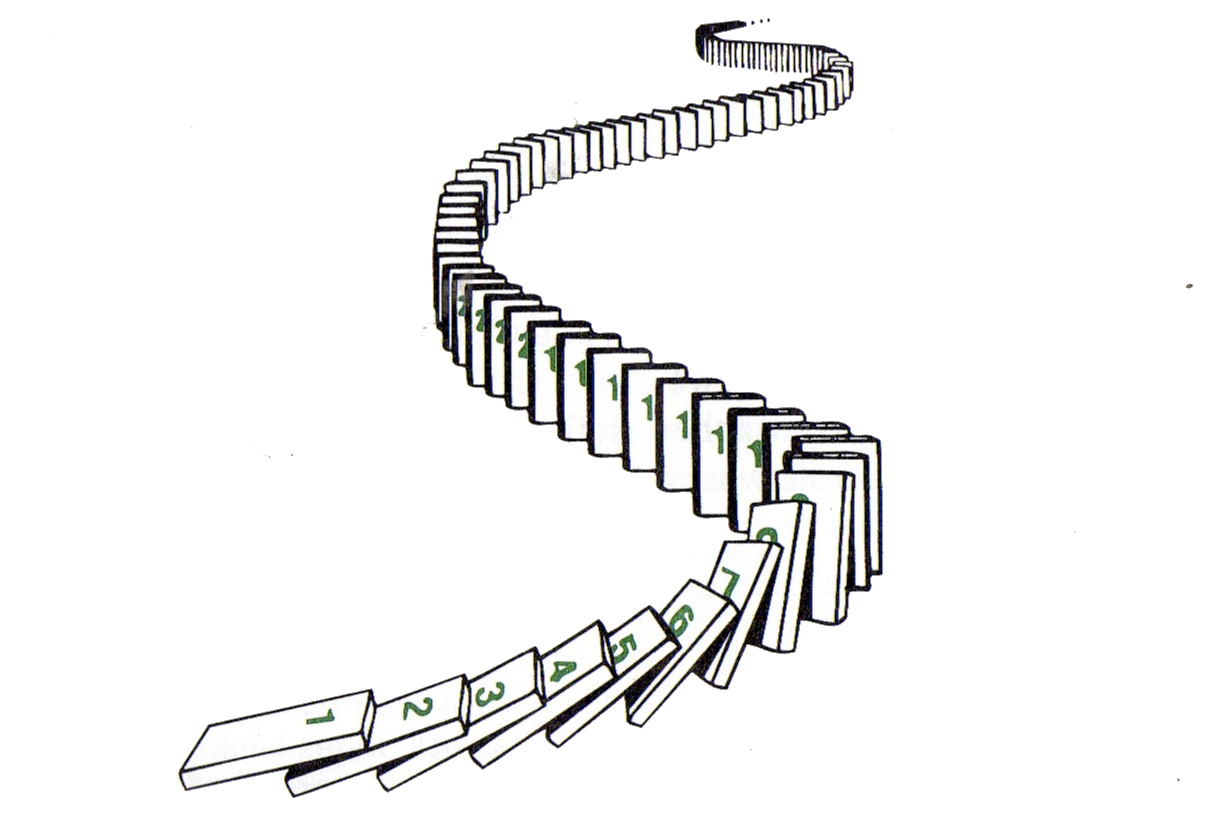
\includegraphics[width=0.4\textwidth]{Figures/domino.png}
    \caption{Ilustración del principio de inducción.}
\end{figure}
Esta técnica se puede visualizar como una fila de fichas de dominó: si la primera ficha cae y si al caer una ficha hace caer la siguiente, entonces todas las fichas caerán.


\begin{exampleblock}{Ejemplo: Suma de los primeros números naturales}
Probaremos por inducción que:
$$ 0 + 1 + \dots + n = \frac{n(n+1)}{2}. $$

\textbf{Caso base:} Para $n=0$, tenemos $0 = \frac{0(0+1)}{2}$, que es cierto.

\textbf{Caso inductivo:} Supongamos que la fórmula es válida para algún $n$, es decir,
$$ 0 + 1 + \dots + n = \frac{n(n+1)}{2}. $$

Queremos demostrar que también se cumple para $n+1$:
\begin{align*}
    0 + 1 + \dots + n + (n+1) &= \frac{n(n+1)}{2} + (n+1) \
    &= \frac{n(n+1) + 2(n+1)}{2} \
    &= \frac{(n+1)(n+2)}{2}.
\end{align*}

Por lo tanto, la propiedad se mantiene y queda demostrada por inducción.
\end{exampleblock}

\subsubsection*{Limitaciones del principio de inducción}
La inducción es una técnica muy útil para \alert{probar} versiones cerradas de fórmulas que involucran e.g. sumatorias, productorias o recurrencias, pero no nos dice
nada sobre cómo \alert{inferir} dichas formas cerradas. 

\subsection{Generalización del Principio de Inducción}

En algunas ocasiones, la propiedad que queremos demostrar no necesariamente comienza en $n=0$, sino en un valor inicial diferente, digamos $n_0$. En estos casos, podemos formular una versión más general del principio de inducción:

\begin{definitionblock}{Principio de Inducción Generalizado}
Si queremos demostrar que una propiedad $P(n)$ es válida para todos los números naturales mayores o iguales a un cierto $n_0$, basta con probar:
\begin{itemize}
    \item \textbf{Caso base:} Se demuestra que la propiedad es cierta para $n = n_0$.
    \item \textbf{Caso inductivo:} Se asume que la propiedad es cierta para un número arbitrario $n \geq n_0$ (hipótesis inductiva) y se demuestra que también es cierta para $n+1$.
\end{itemize}

Simbólicamente,
$$ P(n_0) \wedge \forall n \geq n_0 \; (P(n) \rightarrow P(n+1)) \Rightarrow \forall n \geq n_0. P(n). $$
\end{definitionblock}

Esta generalización es útil cuando la propiedad que queremos demostrar solo tiene sentido a partir de cierto número natural. Por ejemplo, si estamos probando una afirmación sobre la factorización de números naturales en factores primos, podríamos necesitar que el primer caso considerado sea $n_0 = 2$, ya que el número 1 no es primo ni compuesto.

\subsection*{Ejercicio: Lanzamiento de Pelotas en el Parque}
Un número impar de personas está de pie en un parque, cada una con una pelota en la mano. La distancia entre cualquier par de personas es distinta.

Cada persona lanza su pelota a la persona que está más cerca de ella. Queremos demostrar por inducción que \textbf{siempre existe al menos una persona que no recibe ninguna pelota}.

\medskip

Usando inducción, demostraremos la siguiente proposición \( P(n) \) sobre los números naturales mayores o iguales a 1:

\medskip

\begin{center}
  \( P(n) ~~\equiv~~ \)  Cuando en el parque se paran \( 2n+1 \) personas, existe una que no recibe ninguna pelota.
\end{center}
% \medskip

\subsubsection*{Caso base: \( P(1) \)}

Entre las tres personas, sean \( A \) y \( B \) las que están separadas por la menor distancia y \( C \) la persona restante, es decir:
\[
  d(A,B) < d(A,C) \quad \text{y} \quad d(A,B) < d(B,C).
\]

Como consecuencia, \( A \) y \( B \) se lanzan la pelota mutuamente, y por lo tanto, \( C \) no recibe ninguna pelota.

% \begin{figure}[h]
%     \centering
%     
\includegraphics[width=0.2\textwidth]{Figures/ejercicio_induccion.png}
%     \caption{Ilustración del juego de pelotas en el parque.}
% \end{figure}

\subsubsection*{Caso inductivo}

Supongamos por hipótesis inductiva que en un grupo de \( 2n+1 \) personas siempre hay alguien que no recibe ninguna pelota. 
Queremos demostrar que lo mismo ocurre para \( 2n+3 \) personas.

Sean \( A \) y \( B \) las personas que están separadas por la menor distancia. Como en el caso base, \( A \) y \( B \) se lanzan la pelota mutuamente.

Ahora analizamos los siguientes casos:

\begin{itemize}
    \item Si alguien más le lanza su pelota a \( A \) o a \( B \), entonces el máximo de pelotas recibidas entre los restantes \( 2n+1 \) participantes es \( 2n \), y por tanto, al menos uno de ellos no recibe ninguna pelota.
    
    \item Supongamos que la única pelota que recibe \( A \) es la de \( B \), y viceversa. El resto del grupo es de \( 2n+1 \) personas, y todas las distancias entre ellas son distintas. Por hipótesis inductiva, alguien en este grupo no recibe ninguna pelota.
\end{itemize}

Por lo tanto, la proposición se mantiene para \( 2n+3 \), y el principio de inducción nos permite concluir que siempre habrá una persona que no recibe ninguna pelota en cualquier número impar de participantes.


\subsection{Ejercicios propuestos}

\begin{itemize}
    \item Demuestre que si $h > -1$, entonces para todo entero no negativo $n$ se tiene que $1+nh \leq (1+h)^n$.
    \item Demuestre que para todo entero positivo $n$ se tiene que $\sum_{i=1}^n \frac{1}{\sqrt{i}} > 2(\sqrt{n+1}-1)$.
    \item Sean $a_1,a_2,\dots,a_n$ números reales positivos. Probar que $$\frac{1}{n} (a_1+a_2+ \cdots + a_n) \geq (a_1 a_2 \cdots a_n)^{\frac{1}{n}}.$$ \end{itemize}


\section{Principio de Inducción Fuerte}
% \section{Simplificando el Caso Inductivo}

En el caso inductivo, para probar $P(n+1)$ sólo podemos emplear $$P(n)$$

Sin embargo, muchas pruebas se simplifican significativamente si pudiésemos emplear
$$P(0) \:\land\: P(1) \:\land\: \ldots \:\land\: P(n)$$

Este último argumento de prueba es válido y se conoce como \textbf{principio de inducción fuerte}.



\begin{definitionblock}{Principio de Inducción Fuerte}
Una propiedad vale para todos los números naturales si:

\begin{description}
\item[Caso base:] la propiedad vale para $0$.
\item[Caso inductivo:] cualquiera sea el natural $n$, la propiedad vale para $n+1$ si
  vale para todos los naturales menores o iguales a $n$.
\end{description}

Simbólicamente,
$$P(0) \,\wedge\, \forall n \;  ( P(0) \land P(1) \land \ldots \land P(n) ) \rightarrow P(n+1) \ \ \ 
\rightarrow \ \ \ \forall n.\ P(n)$$
\end{definitionblock}


\subsection{Ejercicio: Descomposición en Factores Primos}

Pruebe por inducción fuerte que todo natural mayor que 1 puede escribirse como producto (posiblemente unitario) de factores primos.

\textbf{Caso base:} Trivial ya que $2$ puede escribirse como el producto unitario $2$.

\textbf{Caso inductivo:} Considere el natural $n+1$ y asuma por hipótesis inductiva que todo natural en el intervalo $[2, n]$ puede escribirse como producto de factores primos. Ahora analicemos si $n+1$ es primo o compuesto.

\begin{itemize}
\item Si $n+1$ es primo, la propiedad es trivial.
\item Si $n+1$ es compuesto, entonces existen naturales $j,k$ en el intervalo $[2,n]$ tales que $n+1 = j \cdot k$. Por hipótesis inductiva, $j$ y $k$ pueden escribirse como producto de factores primos, y por lo tanto $n+1=j\cdot k$ también.
\end{itemize}

\textbf{Observación:} Para esta prueba usamos la variante del principio de inducción fuerte que establece la propiedad respectiva a partir de $2$ (no a partir de 0).



\subsection{Ejercicio: Cortando Barras de Chocolate}
\begin{wrapfigure}{r}{0.3\textwidth}
    \centering
    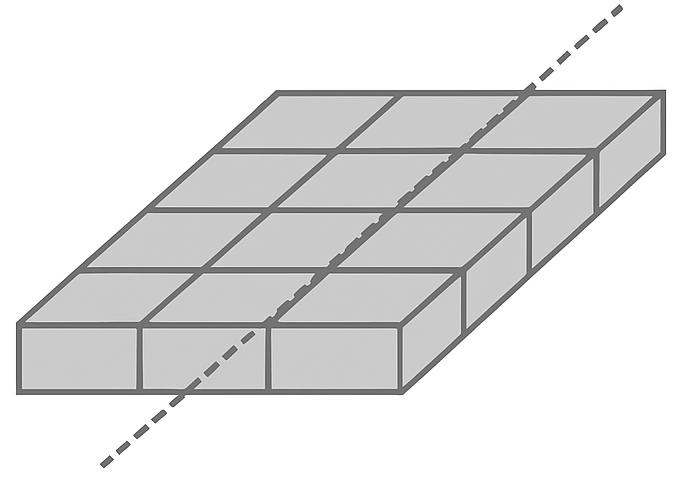
\includegraphics[width=0.22\textwidth]{Figures/barra.png}
    % \caption{Ilustración del principio de inducción.}
\end{wrapfigure}
Una barra de chocolate consiste en $m \times n$ cuadrados dispuestos en $m$ filas y $n$ columnas. Uno puede partir la barra en cuadrados  cortándola a lo largo de sus ``lineas''. Asumiendo que las lineas no se pueden cortar parcialmente, demuestre que $mn - 1$ cortes  alcanzan para obtener los  $mn$ cuadrados.

Haremos la demostración por inducción fuerte sobre el número $k=mn$ de cuadrados de la barra de chocolate.

\textbf{Caso base:} Una barra de $k=1$ cuadrado trivialmente puede ser cortada en cuadrados con $1-1$ cortes.

\textbf{Caso inductivo:} Consideremos una barra de $k+1$ cuadrados. Hagamos sobre la barra un corte arbitrario. Éste divide a la barra en dos subbarras de $k_1$ y $k_2$ cuadrados respectivamente, donde $k_1 + k_2 = k+1$.

Por hipótesis de inducción estas dos barras pueden ser cortadas con $$k_1 - 1 \quad \text{y} \quad k_2-1$$ cortes. Por tanto, la barra original (de $k+1$ cuadrados) puede cortarse con:
\begin{align*}
    1 \; + \; k_1 - 1  \; + \; k_2 - 1 &= k_1 + k_2 -1 \\
    &= k
\end{align*}

cortes. Así se demuestra que cualquier barra de chocolate de $mn$ cuadrados puede ser cortada en unidades utilizando exactamente $mn - 1$ cortes.

\section{Comparando los dos principios de inducción}

Los dos principios de inducción estudiados (el estándar---también llamado \emph{débil}---y el fuerte) son \textbf{igualmente expresivos}. Esto significa que una propiedad puede ser establecida usando uno si y sólo si puede ser establecida usando el otro. 

Ambos principios permiten demostrar afirmaciones sobre los números naturales, pero en algunos casos el uso del principio de inducción fuerte simplifica considerablemente la demostración, ya que en lugar de depender solo de \( P(n) \) para demostrar \( P(n+1) \), permite utilizar todas las propiedades anteriores \( P(0), P(1), ..., P(n) \).

\medskip
\medskip

\textbf{Ejercicio:} Derive el principio de inducción fuerte a partir del principio de inducción estándar. \textit{Hint:} Proceda por inducción.

% \textbf{Demostración: Derivación del Principio de Inducción Fuerte a partir del Principio de Inducción Estándar}

% Para demostrar que el principio de inducción fuerte se sigue del principio de inducción estándar, procedemos por inducción sobre \( n \):

% \begin{itemize}
%     \item \textbf{Caso base:} Para \( n=0 \), la hipótesis de inducción estándar nos garantiza que \( P(0) \) es cierto.
    
%     \item \textbf{Paso inductivo:} Supongamos que el principio de inducción estándar es válido y que se cumple que \( P(n) \rightarrow P(n+1) \). Queremos demostrar que el principio de inducción fuerte también es válido, es decir, que si \( P(0), P(1), ..., P(n) \) son verdaderos, entonces también lo es \( P(n+1) \).
    
%     Como el principio de inducción estándar garantiza que \( P(n) \) implica \( P(n+1) \), podemos ver que, si asumimos que todos los valores anteriores hasta \( P(n) \) son ciertos, entonces \( P(n+1) \) también debe serlo, ya que el último paso de la demostración depende exclusivamente de \( P(n) \), el cual hemos supuesto verdadero.
    
%     Por lo tanto, el principio de inducción fuerte es una consecuencia directa del principio de inducción estándar.
% \end{itemize}

\subsection{Principio del Buen Orden}

El principio del buen orden es un concepto fundamental en la teoría de números y es equivalente al principio de inducción. Nos dice que cualquier subconjunto no vacío de los números naturales tiene un elemento mínimo. Esto significa que no existen secuencias infinitamente decrecientes en los naturales.

\begin{definitionblock}{Principio del Buen Orden}
Sea \( S \) un subconjunto no vacío de los números naturales \( \mathbb{N} \). Entonces, existe un elemento mínimo \( m \in S \), es decir, un número \( m \) tal que para todo \( x \in S \), se cumple que \( m \leq x \).
\end{definitionblock}

El principio del buen orden es la base lógica de la inducción matemática, ya que podemos utilizarlo para demostrar el principio de inducción estándar por reducción al absurdo. La idea detrás de esta prueba es suponer que existe un número natural para el cual no se cumple la propiedad que queremos demostrar, y mostrar que esto lleva a una contradicción con el principio del buen orden.

\medskip
\medskip

\textbf{Ejercicio:} Derive el principio de inducción estándar a partir del principio del buen orden. \textit{Hint:} Proceda por reducción al absurdo.

% \textbf{Demostración: Derivación del Principio de Inducción Estándar a partir del Principio del Buen Orden}

% Supongamos que el principio de inducción estándar no es cierto. Es decir, existe un subconjunto de los números naturales \( S \) tal que:
% \begin{itemize}
%     \item Contiene todos los valores para los cuales la propiedad \( P(n) \) no es verdadera.
%     \item Este conjunto \( S \) es no vacío.
% \end{itemize}

% Por el principio del buen orden, sabemos que \( S \) tiene un elemento mínimo, digamos \( m \). Es decir, \( P(m) \) no es cierto, pero para todo número menor que \( m \), la propiedad sí se cumple.

% Ahora bien, por la hipótesis de inducción estándar, si \( P(k) \) es cierto para algún \( k \), entonces \( P(k+1) \) también lo es. Como todos los números menores que \( m \) cumplen \( P(n) \), se sigue que \( P(m) \) también debe cumplirse, lo cual es una contradicción.

% Por lo tanto, \( S \) debe ser vacío, lo que implica que el principio de inducción estándar es válido.


\medskip
\medskip

Es más, puede probarse que el principio de inducción débil, el principio de inducción fuerte y el principio del buen orden resultan \textbf{equivalentes}. En otras palabras, si se asume cualquiera de estos principios como cierto, se pueden demostrar los otros dos.

